\chapter{Wstęp}
\section{Wprowadzenie}
Świat gier komputerowych, w szczególności gier prowadzonych w trybie \emph{on-line}, budowany jest zwykle w oparciu o różnego rodzaju mechanizmy rywalizacji. Dzięki tym mechanizmom samo granie przestaje mieć formę beztroskiej rozrywki, a staje się czymś więcej -- sposobem na sprawdzenie własnych możliwości, testem osiągniętej sprawności, okazją do zbudowania pozycji itp. Od wprowadzonych zasad oraz zakresu obsługiwanych możliwości interakcji między graczami zależy, czy grono użytkowników danej gry powiększać się będzie o kolejne grupy fanów, czy wręcz przeciwnie, dana gra nie zdobędzie żadnej popularności. Niespecjalnie to nawet dziwi, gdyż rywalizacja jest uważana za część ludzkiej egzystencji, zaś uczestnictwo w cyfrowych konfliktach to tylko realizacja głęboko zakorzenionej potrzeby.

Wydawaniu gier komputerowych niezmiennie towarzyszy tworzenie się wokół nich lokalnych społeczności, zrzeszających osoby o podobnych zainteresowaniach. Przykładem takiej społeczności jest, ciesząca się zasłużoną renomą, społeczność FGC (ang.~\emph{Fighting Game Community}). Jej członkowie, włącznie z autorem niniejszej pracy, rywalizują ze sobą, dzielą się wskazówkami, transmitują swoje rozgrywki oraz, co równie istotne, budują nowe relacje przyjacielskie. Dla wielu z nich udział w turniejach to nie tylko okazja do rywalizacji, ale także pretekst do spotkania ze starymi znajomymi dzielącymi tę samą pasję.

Pojawiający się w angielskiej nazwie grupy termin \emph{Fighting Games} wskazuje na pewien gatunek gier, wokół których skupia się ta społeczność. W tłumaczeniu na język polski tego typu gry określa się mianem ,,bijatyk''. W  ,,bijatykach'' rywalizacja pomiędzy graczami odbywa się na wzór rywalizacji w sztukach walki -- gracze wykonują ruchy awatarami, zadając sobie ciosy, blokując ataki i stosując uniki. Cała rozgrywka obywa się w wirtualnym świecie o różnej złożoności, od dwuwymiarowej sceny, poprzez rozbudowane mapy, aż po trójwymiarowe środowiska renderowane z dokładnością bliską filmowanej rzeczywistości.

Wspomniane kulturowe otoczenia bijatyk, jak również budowany od dzięcięcych lat sentyment do tego typu gier, okazały się kluczowymi czynnikami do zdefiniowania i podjęcia przez autora tematu niniejszej pracy dyplomowej. Jego realizacja, ujmując to w skrócie, polegać ma na stworzeniu sieciowej gry z gatunku bijatyk, oferującej prostą, dwuwymiarową wizualizację sceny oraz proste sterowanie.

Dobrym przykładem ilustrującym działanie gier z gatunku bijatyk jest gra FOOTSIES: \url{https://store.steampowered.com/app/1344740/FOOTSIES_Rollback_Edition/}. 
% TO DO: można tutaj opisać tę grę nieco szerzej, dodajaś zrzuty ekranu oraz opisy "ciosów". Chodzi o to, by było wiadomo, jak wygląda bijatyka 2D.
Na rysunku~\ref{fig:footsies} pokazano jeden z głównych widoków prezentowanych uczestnikom gry, zaznaczając na nim główne jego elementy. Widok ten ma ułatwić zrozumienie, o czym będzie niniejsza praca. 
\begin{figure}
	\centering
		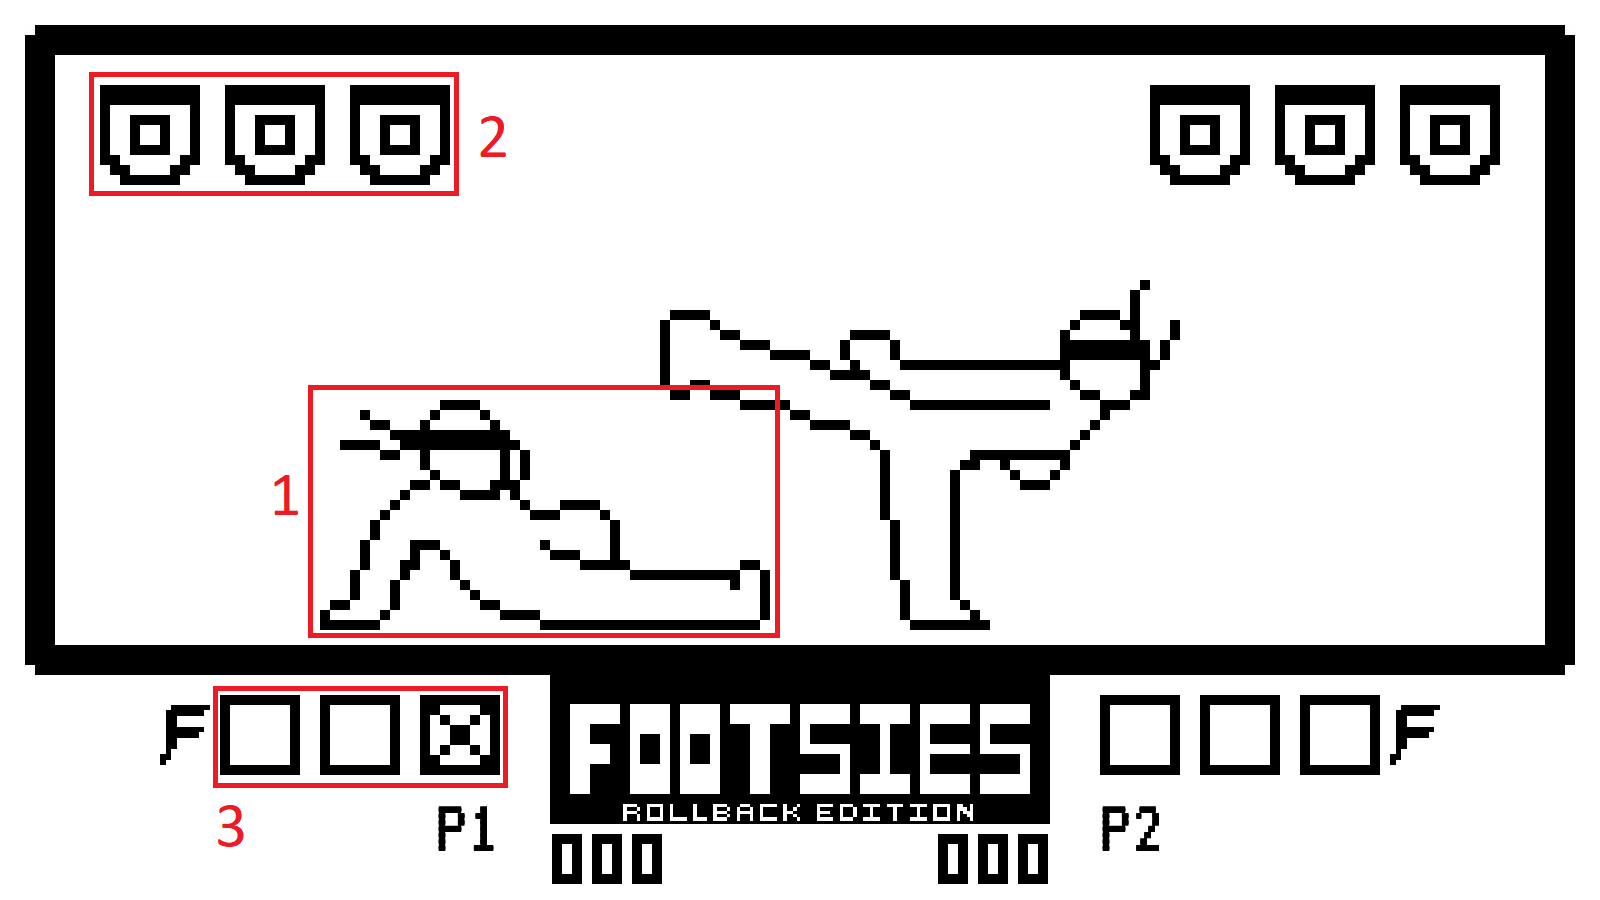
\includegraphics[width=0.64\linewidth]{rys01/footsies}
	\caption{Zrzut ekranu z gry FOOTSIES z zaznaczonymi głównymi elementami gry: 1 - postać którą steruje gracz, 2 - licznik punktów bloku, 3 - licznik wygranych rund}
	\label{fig:footsies}
\end{figure}

Jak można się domyślać, gracz kontroluje reprezentującą go postać (awatara), rywalizując z innym graczem (z jego awatarem) w kolejnych rundach. Celem danej rundy jest powalenie przeciwnika. Kto tego dokona, wygrywa daną rundę. Wygranie trzech rund oznacza zwycięstwo w całej grze (i jej zakończenie).

Gracze mają możliwość wykonywania różnych ruchów. Mogą na przykład przemieszczać awatara po planszy, poruszając nim w stronę przeciwnika lub cofając go. Warto zaznaczyć, że cofanie pozwala zablokować nadchodzące ataki. Odbywa się to jednak kosztem utraty punktów bloku. Wyzerowanie konta punktów bloku sprawia, że dana postać awatara staje się bezbronna.

Jeśli chodzi o ataki, to wyróżnia się ich dwa główne: ataki normalne i ataki kończące. Atak normalny jest stosunkowo szybki, co może okazać się przydatne, jako że podczas animacji jakiegokolwiek ataku nie możemy blokować. Służy on głównie do testowania przeciwnika i zmniejszania jego punktów bloku. Każdy normalny atak ma kontynuację w postaci ataku kończącego. Jeśli uda się trafić przeciwnika atakiem kończącym, przeciwnik przewraca się, a to oznacza zwycięstwo w rundzie. Ataki kończące są znacznie wolniejsze i odsłaniają postać atakującego na odpowiedź przeciwnika (jest wystarczająco dużo czasu, aby przeciwnik zadał kontrujący atak kończący). Do tego dochodzą dodatkowe właściwości poszczególnych ciosów, jak np.\ niewrażliwość na ciosy przeciwnika podczas animacji.

Cała mechanika gry pozwala na wdrożenie interesujących strategii. Mogą one obejmować próby zmylenia przeciwnika i skłonienia go do podjęcia złego ruchu, zazwyczaj poprzez stworzenie sytuacji, która wskazuje na zamiar zrobienia jakiegoś konkretnego ruchu, gdy faktycznie w planach atakującego jest coś innego. Przykładowo, \emph{whiff punishing} to jeden z elementów taktyki polegającej na kontrolowaniu odległości w trakcie walki. Konkretnie oznacza on skaranie przeciwnika za chybienie podczas swojego ataku. Idea wykorzystująca tę taktykę może polegać na zbliżeniu się do przeciwnika w taki sposób, aby zachęcić go do podjęcia ataku, a następnie szybko się cofnąć, obserwując, jak przeciwnik popełnia błąd i skontrować go. 

% TO DO: przypominam (na przyszłość), że do każdego rysunku musi istnieć w tekście jakiś opis oraz referencja


\section{Cel i zakres pracy}
Celem niniejszego projektu jest opracowanie oraz pełna implementacja dwuwymiarowej gry zręcznościowej, zaliczającej się do kategorii bijatyk. Gra ta ma umożliwiać rywalizację pomiędzy graczami w trybie online, przy wykorzystaniu uproszczonych rozwiązań w zakresie sterowania, grafiki i mechaniki walki.

Realizacja pracy rozpocznie się od zdefiniowania wymagań. Ważne na tym etapie będzie zwrócenie uwagi na możliwe ścieżki implementacji gry. Następnie, po dokonaniu wybooru odpowiedniej technologii i konfiguracji środowiska programistycznego, nastąpi etap projektowania i implementacji. W ramach tej części pracy zostanie stworzony interfejs użytkownika oraz opracowana mechanika rozgrywki. Kolejnym krokiem będzie napisanie kodu źródłowego oraz stworzenie grafik. Cały projekt zostanie poddany szeregowi testów celem zapewnienia jego poprawnej działalności. Ostatecznie zostanie przygotowana pełna dokumentacja projektu, włączając w nią instrukcję obsługi.

\section{Układ pracy}
W rozdziale pierwszym przedstawiono wprowadzenie do tematu gier z gatunku bijatyk, oraz zakres, cel i układ pracy.
W rozdziale drugim opisano założenia projektowe.
W kolejnym, trzecim rozdziale, przedstawiono szczegóły implementacji, łącznie z opisem fragmentów kodu źródłowego.
W rozdziale czwartym zwrócono uwagę na testy oraz uzyskane wyniki.
Ostatni, piąty rozdział, przeznaczono na podsumowanie.
Pracy towarzyszy wykaz literatury oraz dwa dodatki. 

